\documentclass[a4paper]{article}
\usepackage[utf8]{inputenc}
\usepackage[T1]{fontenc}
\usepackage[english]{babel}
\usepackage{amsmath,amsthm,amsfonts,amssymb, mathtools}
\usepackage{mathtools}
\usepackage{mathrsfs}
\usepackage[a4paper,margin=3cm]{geometry}
\usepackage{bm}
\usepackage{tikz}
\usetikzlibrary{calc,arrows,fadings, automata, positioning}
\tikzfading[name=fade inside,inner color=red,outer color=blue]

\title{How did the Ever Given get stuck in the Suez canal?}


\author{Miguel De Le Court}
\date{June 2021}

\begin{document}
\maketitle

\vfill

\begin{abstract}
    This reports aims at studying the 2021 Suez canal incident with a 2d CFD model. We start by reconstructing the historical events using a siplified geometry for the canal and the ship. We then formulate an ALE FEM model where the mesh follows the boat in space, and use it to compute the forces on the ship. We then use this data to reproduce the events without enforcing the movements a priori. Based on a slightly tweaked simulation, we show that the incident likely could have been avoided if teh ship had been controlled slightly differently. We also point out at the difficulty of finding such ship controls, due to some positive feedback loops that happen when steering the ship.
\end{abstract}
\vfill

\newpage
\section{Introduction}
\subsection{Background and Research question}
In March 2021, the Suez Canal was blocked for six days after the Ever Given container ship got stuck sideways in the canal. The Suez canal is route to about 12\% of global trade, and it is estimated that the blockade cost around \$9 Billion per day\cite{bbc:cost}\cite{bbc:cost2}\cite{guardian:cost}. To this day, the effect of the incident are still affecting some parts of the economy\cite{consequ1}\cite{consequ2}, thus, understanding the causes of this incident may be of a crucial importance. 

One known effect that played a significant role in the incident, and which is the most common explaination for it, is the so-called bank effect. When a ship moves forward, an area of high pressure is created around bow of the ship. The water that flows along its sides will, on the contrary, create a low pressure area. When the ship is close to a vertical obstacle, such as the bank, the pressure gradient will produce a couple of forces that will tend to stir the ship\cite{bankeffect}, as shown below. While the bank effect qualitatively explains the movements of the ship around $t=7$ minutes in Figure \ref{fig:snaps}, it is not sufficient to explain what happened previously.


\begin{center}
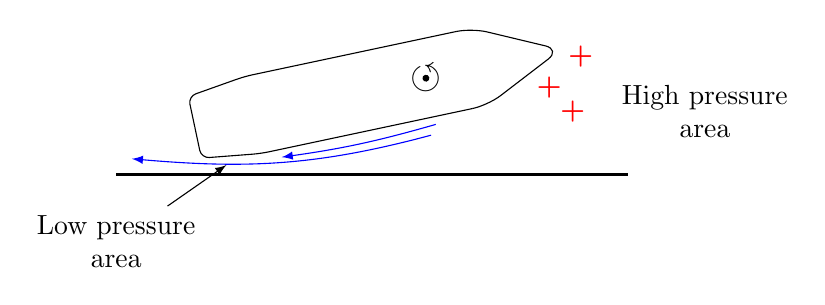
\begin{tikzpicture}
    \begin{scope}[shift={(1,0.6)}, rotate=12, scale=0.5]
        \draw[rounded corners=1mm] (0,0)  -- (0, -0.8) -- (1.5,-1) -- (7,-1);
        \draw[rounded corners=1mm] (0,0)  -- (0, 0.8) -- (1.5,1) -- (7,1);
        \draw[rounded corners=2mm] (7, -1) -- (7.4, -1) -- (9.5, 0) -- (7.4, 1)  -- (7,1);
        \draw [blue, -latex] (6, -1.2) to [bend left=4] (2, -1.2);
        \node at (6,0) (P) {\Large $\circlearrowleft$};
        \fill (6, 0) circle[radius=2.5pt];
    \end{scope}

    \draw[thick] (0,0) -- (6.5,0);
    \draw [blue, -latex] (4,0.5) to[out=195,in=-5] (0.2,0.2);
    \node[red] at (5.5, 1.1) {$\bm{+}$};
    \node[red] at (5.9, 1.5) {$\bm{+}$};
    \node[red] at (5.8, 0.8) {$\bm{+}$};
    \node[right, align=center] at (6.3, 0.8) (nhp) {High pressure\\ area};
    \node[below, align=center] at (0, -0.4) (nlp) {Low pressure\\ area};
    \draw[-latex] (nlp) -- (1.4,0.12);
\end{tikzpicture}    
\end{center}

This project will thus consist in simulating canal obstruction and some other variations on what happened. The goals are to understand why the Ever given got stuck, and what forces were present. We expect to observe and quantify the bank effect at around $t=7$ minutes in Figure \ref{fig:snaps}. We also whish to explain the reasons why the ship got this close to the shore in the first place. With the study of the the typical forces, we also want to highlight possible feedback loops that happen when navigating in a restricted space with a large ship.

\begin{figure}[hbtb]
    \centering
	\includegraphics[width=\textwidth]{Figures/snaps.pdf}
	\caption{Snapshots of the ship positions during the incident}
	\label{fig:snaps}
\end{figure}



\subsection{State of the art}
This project mainly focuses on the study of the fluid forces on a solid, and the interactions that the solid and fluid have. Since the ship will be moving forward during most of the simulation, we will need to move the domain accordingly\footnote{Or use a very large domain for the simulation but this is not the option that was retained.}. These two reasons naturally lead to the choice of using an ALE FEM model that moves along the ship vertically, and deforms to accomodate the rotations and lateral movements. ALE models are commonly used to simulate problems where fluid-structure interaction is of key interest\cite{Jeannette2020Apr}\cite{Wang2018Jul} due to their great interface capturing capabilities. Solids are described in a Lagrangian framework, while the Eulerian framework is most often used for fluids. The solid deformation is computed in a Lagrangian framework and then the mesh is moved using some kind of smoothing that aims at maintaining a reasonable mesh quality for the fluid.  The main challenge with ALE-FEM occurs when large deformations require remeshing to maintain an acceptable mesh quality, or changing the mesh topology. The solution to this problem involves re-meshing globally or locally, and projecting the solution on the new mesh\cite{Remacle2010May}. The main drawbacks of a global remshing is that the projection of the solution onto the new mesh introduces a lot of numerical diffusion. This is made even worse when we whish to keep a divergence-free field from one mesh to another, as it either adds constraints on the projection, or like in this report, produces unphysical behaviours\footnote{In this context those would be extremely strong pressure gradients.} that may take some time to recover. Another drawback is that a global remeshing is difficult to apply in parallel. Local remeshing like done in \cite{Remacle2010May}, on the other had, requires a rather low level interaction with the mesh generation algorithm, whish was not easyly feasible with dolfin.

\section{Method}



\newpage
\bibliographystyle{IEEEtran}
\bibliography{biblio.bib}
\end{document}
